\section{Bilder}
\begin{figure}[H]
    \centering
    \caption[]{Mockup der Übersicht}\label{fig:MockupOverview}
    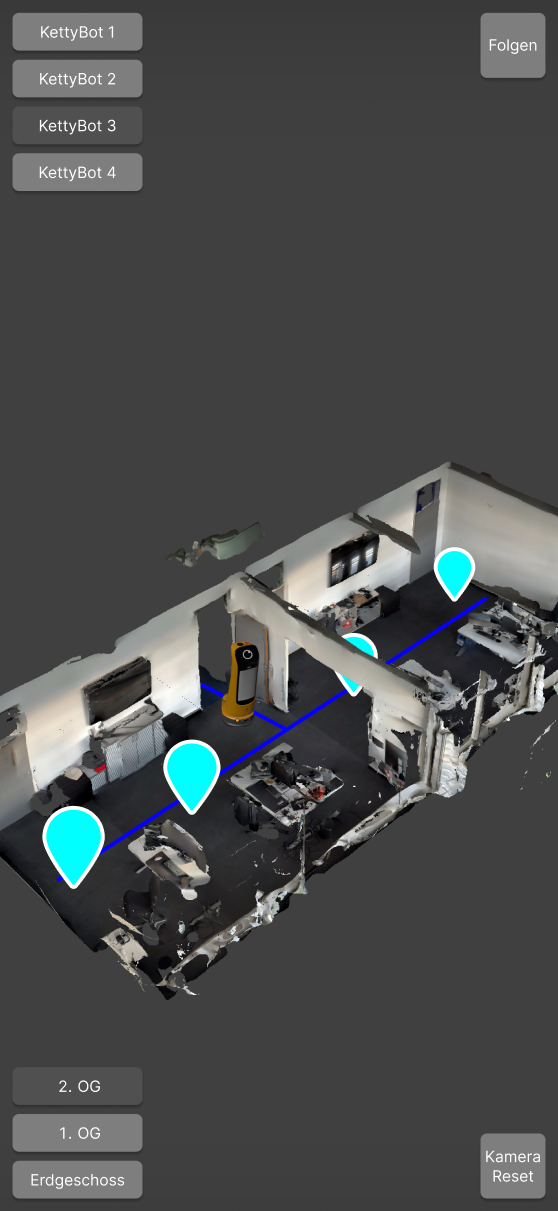
\includegraphics[width=0.5\textwidth]{Mockup Uebersicht}
    \\
    Quelle: Eigene Darstellung
\end{figure}

\begin{figure}[H]
    \centering
    \caption[]{Mockup der Steuerung}\label{fig:MockupControls}
    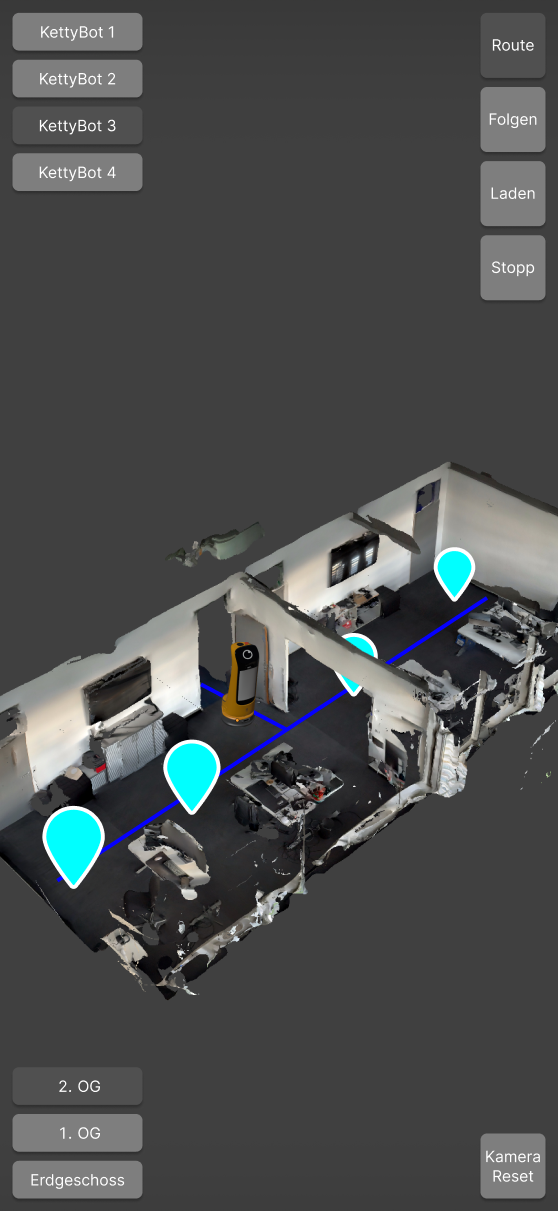
\includegraphics[width=0.5\textwidth]{Mockup Steuerung}
    \\
    Quelle: Eigene Darstellung
\end{figure}

\begin{figure}[H]
    \centering
    \caption[]{Mockup des Routenplanungs-Popup}\label{fig:MockupRoutePlanner}
    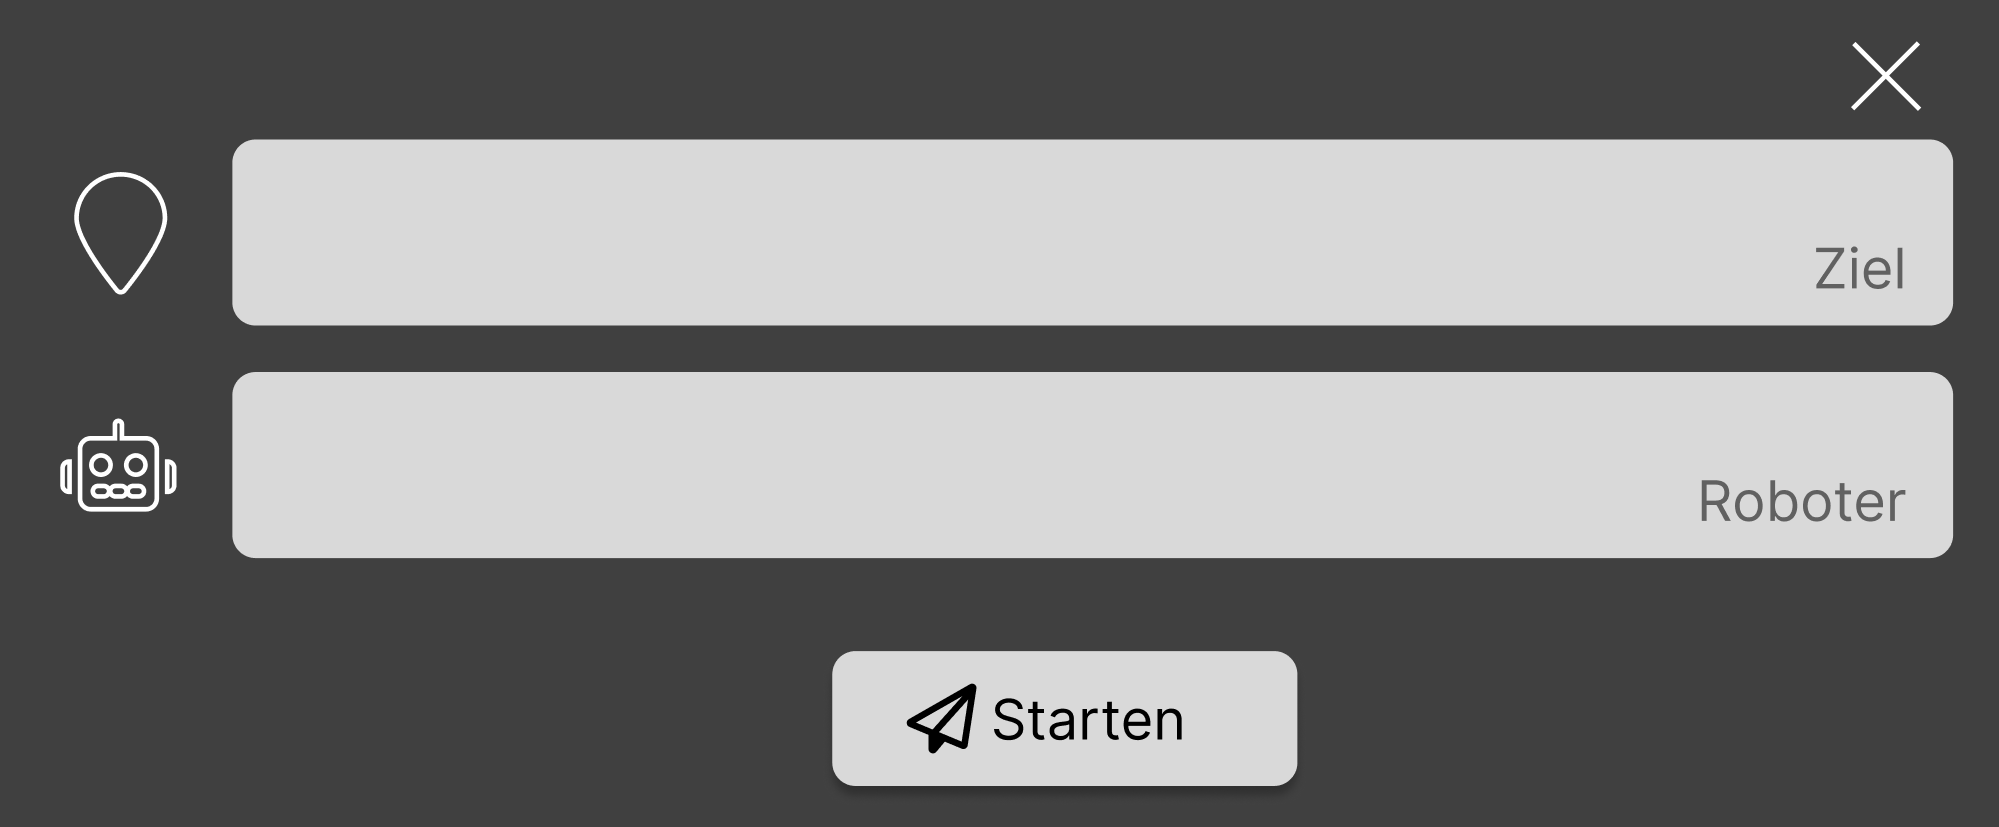
\includegraphics[width=0.9\textwidth]{Mockup Routenplaner}
    \\
    Quelle: Eigene Darstellung
\end{figure}

\begin{figure}[H]
    \centering
    \caption[]{Mockup der Verwaltung}\label{fig:MockupAdministration}
    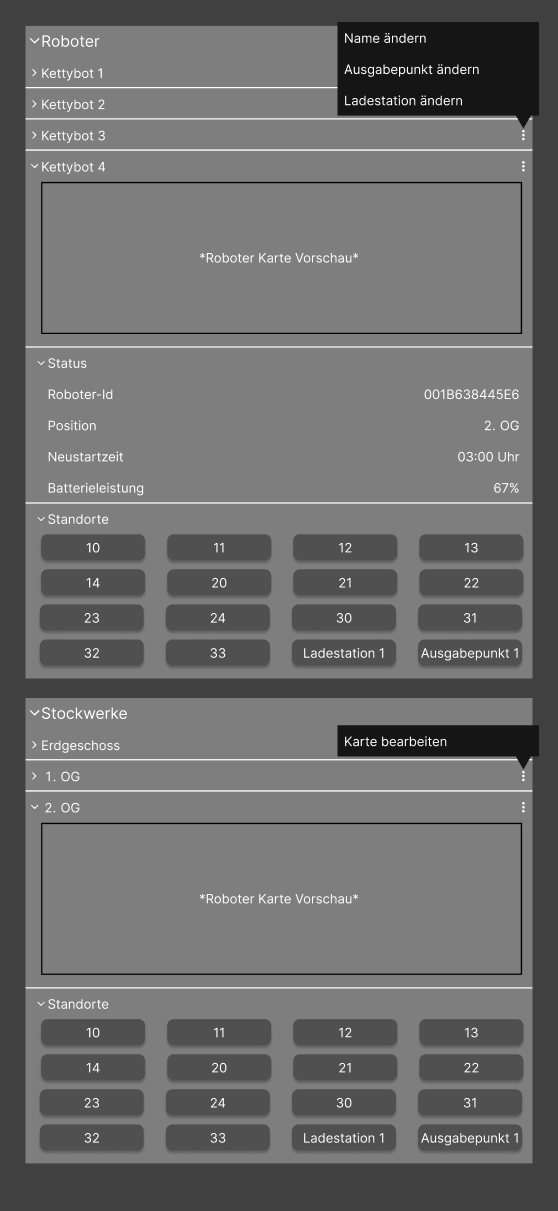
\includegraphics[width=0.5\textwidth]{Mockup Verwaltung}
    \\
    Quelle: Eigene Darstellung
\end{figure}

\section{Tabellen}
\begin{table}[H]
    \caption{Beschreibung der Probleme in erster Usability Test Runde}\label{tbl:1stUsabilityTestsProblemsDesc}
    \begin{tabular}{l|l}
        Problem     & Beschreibung \\ \hline
        Problem 1   & \multicolumn{1}{p{12cm}}{Der Ladestation Button mit Akkustand verwechselt.} \\ \hline
        Problem 2   & \multicolumn{1}{p{12cm}}{Die Icons der Buttons sind nicht selbsterklärend. Ohne anklicken der Buttons kennt man die Funktionen nicht.} \\ \hline
        Problem 3   & \multicolumn{1}{p{12cm}}{Die Anordnung der Ergebnisse im Input Dropdown suggeriert, dass man nur nach Nummern und nicht nach Namen suchen kann.} \\ \hline
        Problem 4   & \multicolumn{1}{p{12cm}}{Die Tooltips auf der Karte sind durch die Farben schlecht lesbar.} \\ \hline
        Problem 5   & \multicolumn{1}{p{12cm}}{Die Fehlermeldungen erklären das Problem nicht.} \\ \hline
        Problem 6   & \multicolumn{1}{p{12cm}}{Es wurde versucht die Modelle in der Übersicht zu verschieben, statt in den Editiermodus zu wechseln.} \\ \hline
        Problem 7   & \multicolumn{1}{p{12cm}}{Erklärung der Steuerung im Editiermodus ist nicht eindeutig genug.} \\ \hline
        Problem 8   & \multicolumn{1}{p{12cm}}{Ohne Loslassen der Maus kann nicht zwischen Verschieben und Rotieren des Modells gewechselt werden.} \\ \hline
        Problem 9   & \multicolumn{1}{p{12cm}}{Es wurde erwartet, dass man in der Routenplanung mehrere Ziele einstellen kann.} \\ \hline
        Problem 10  & \multicolumn{1}{p{12cm}}{Es wurde erwartet, dass die Ladestation in der Routenplanung eingestellt werden kann.} \\ \hline
        Problem 11  & \multicolumn{1}{p{12cm}}{Der Toast Dialog der die Steuerung im Editiermodus wurde nicht angezeigt.} \\ \hline
        Problem 12  & \multicolumn{1}{p{12cm}}{Unklarheit darüber wohin das 3D-Modell verschoben werden muss. Hierbei handelt es sich um ein Problem mit der Aktivität und nicht mit dem Prototyp.} \\ \hline
        Problem 13  & \multicolumn{1}{p{12cm}}{Darstellung der 3D-Modelle sieht kaputt aus.} \\ \hline
        Problem 14  & \multicolumn{1}{p{12cm}}{Ein Stockwerk-Button wird durch das Beta Modus Tag von chayns verdeckt.} \\ \hline
        Problem 15  & \multicolumn{1}{p{12cm}}{Es gab Schwierigkeiten beim Positionieren des Modells.} \\ \hline
        Problem 16  & \multicolumn{1}{p{12cm}}{Der Roboter wurde aufgrund des Icons – das über diesem angezeigt wird – nicht erkannt.} \\ \hline
        Problem 17  & \multicolumn{1}{p{12cm}}{Die Transparenz der Lieferauftrag-Fläche macht Text schlecht lesbar und sieht insgesamt nicht gut aus.} \\ \hline
        Problem 18  & \multicolumn{1}{p{12cm}}{Die Robotersteuerungs-Buttons werden nicht angezeigt, wenn die Routenplanung geöffnet ist.} \\ \hline
        Problem 19  & \multicolumn{1}{p{12cm}}{Es wurde erwartet, dass man nach dem Schließen des Eidtiermodus wieder im Nutzermodus landet.} \\ \hline
        Problem 20  & \multicolumn{1}{p{12cm}}{Der Button zum Zurücksetzen der Kameraposition wurde im Editiermodus nicht gefunden, da dieser an einer anderen Position als in der Übersicht angezeigt wird.} \\
    \end{tabular}
\end{table}
\begin{table}[H]
    \caption{Beschreibung der Probleme in zweiter Usability Test Runde}\label{tbl:2ndUsabilityTestsProblemsDesc}
    \begin{tabular}{l|l}
        Problem     & Beschreibung \\ \hline
        Problem 1   & \multicolumn{1}{p{12cm}}{Unklarheit darüber wie man die Karte rotiert.} \\ \hline
        Problem 2   & \multicolumn{1}{p{12cm}}{Beim Entfernen einer Roboterauswahl, wird in das Stockwerk des Roboters gewechselt, obwohl das nur bei der Auswahl eines Roboters passieren sollte.} \\ \hline
        Problem 3   & \multicolumn{1}{p{12cm}}{Es wurde erwartet, dass man den Roboter über das Ladestations-Icon auf der Karte zur Ladestation schicken kann.} \\ \hline
        Problem 4   & \multicolumn{1}{p{12cm}}{Suchfunktion zum Auswählen eines Standorts nicht gefunden, da das Routenplanungs-Popup nicht geöffnet wurde.} \\ \hline
        Problem 5   & \multicolumn{1}{p{12cm}}{Irritation darüber, dass die Steuerung über einen Tooltip erklärt wird.} \\ \hline
        Problem 6   & \multicolumn{1}{p{12cm}}{Editiermodus nicht im Nutzermodus gefunden, da das Icon des Buttons falsch verstanden wurde.} \\ \hline
        Problem 7   & \multicolumn{1}{p{12cm}}{Editiermodus nicht im Admin-Modus gefunden, da das Kontextmenü übersehen wurde.}
    \end{tabular}
\end{table}
